\documentclass[12pt, a4paper]{article}
\usepackage{import}
\usepackage{preamble}

\title{Equivalent Circuits}
\date{\(10^\mathrm{{th}}\) November 2022}
\author{Lee Farrugia}

\begin{document}
    
\maketitle
\thispagestyle{titlepagestyle}
\pagestyle{mystyle}

\section{Abstract}
yes

\begin{multicols*}{2}

\section{Introduction \& Theoretical Background}
The use of open-ended coaxial probes to measure the complex permittivity is used as it is a non invasive and non destructive to the materials being checked. However, those are not the only advantages this method has, but also due to the way it is utilised it allow for bandwidth measurement and easy sampling \parencite{liao2011accurate}. This method can be used to measure the microwave complex permittivity of dielectric materials including lossy dielectrics. As the relationship between the reflection and transmission is quite complex, the equivalent circuit method is used to simplify the relationship \parencite{stuchly1982equivalent}. This is quite useful when dealing with lossy dielectrics and biological tissues, as the biological tissues are not only made up from one type of material but, multiple types of tissues in one sample. Another example of the use of this method is explored in \cite{zajivcek2006evaluation}, where they discuss the relationship of the the complex permittivity and the transmission of healthy tissues and tumour tissues. They further discuss how this method could be used to image people with non-ionising radiation.

\section{Materials \& Methods}
\subsection{Language and Packages}
Python 3.10.8, Numpy, Pandas, Matplotlib.pyplot \,.
\subsection{Methodology}
\begin{enumerate}
    \item The data provided for both methanol and sodium chloride was imported into the program and each sheet was given its own \mintinline{py}{pandas} data frame.
    \item The average for the real and imaginary parts at each frequency was calculated for each standard material, i.e. air, short, di-ionised water.
    \item The averages calculated in the previous were used to calculate the \(\rho\) of each material. These were then used to calculate the \(\Delta\)s found the equation.
    \item The equation used was:
            \begin{equation}
                \varepsilon_m = -\frac{\Delta_{m2}\Delta_{13}}{\Delta_{m1}\Delta_{32}}\varepsilon_3 - \frac{\Delta_{m3}\Delta_{21}}{\Delta_{m1}\Delta_{32}}\varepsilon_1
            \end{equation}
    \item The average for the real part and imaginary part of the data for the complex permittivity was calculated.
    \item The obtained values for the complex permittivity and the averages of the data given were plotted against each other.
    \item Specific points of the data were printed in order to be compared to each other.
\end{enumerate}

\section{Results \& Discussion}
In \cite{marsland1987dielectric} the error correction was described as follows:
\begin{itemize}
    \item Calculate \textbf{E}.
    \item Use the calculated \textbf{E} to correct subsequent error that arise from the measurements.
\end{itemize}
However, as \textbf{E} is not necessary one can substitute the three known admittance values(of air, short and de-ionised water) along with their respective reflective-coefficient thus, cancelling out the \textbf{E} terms.

\begin{figure}[H]
    \centering
    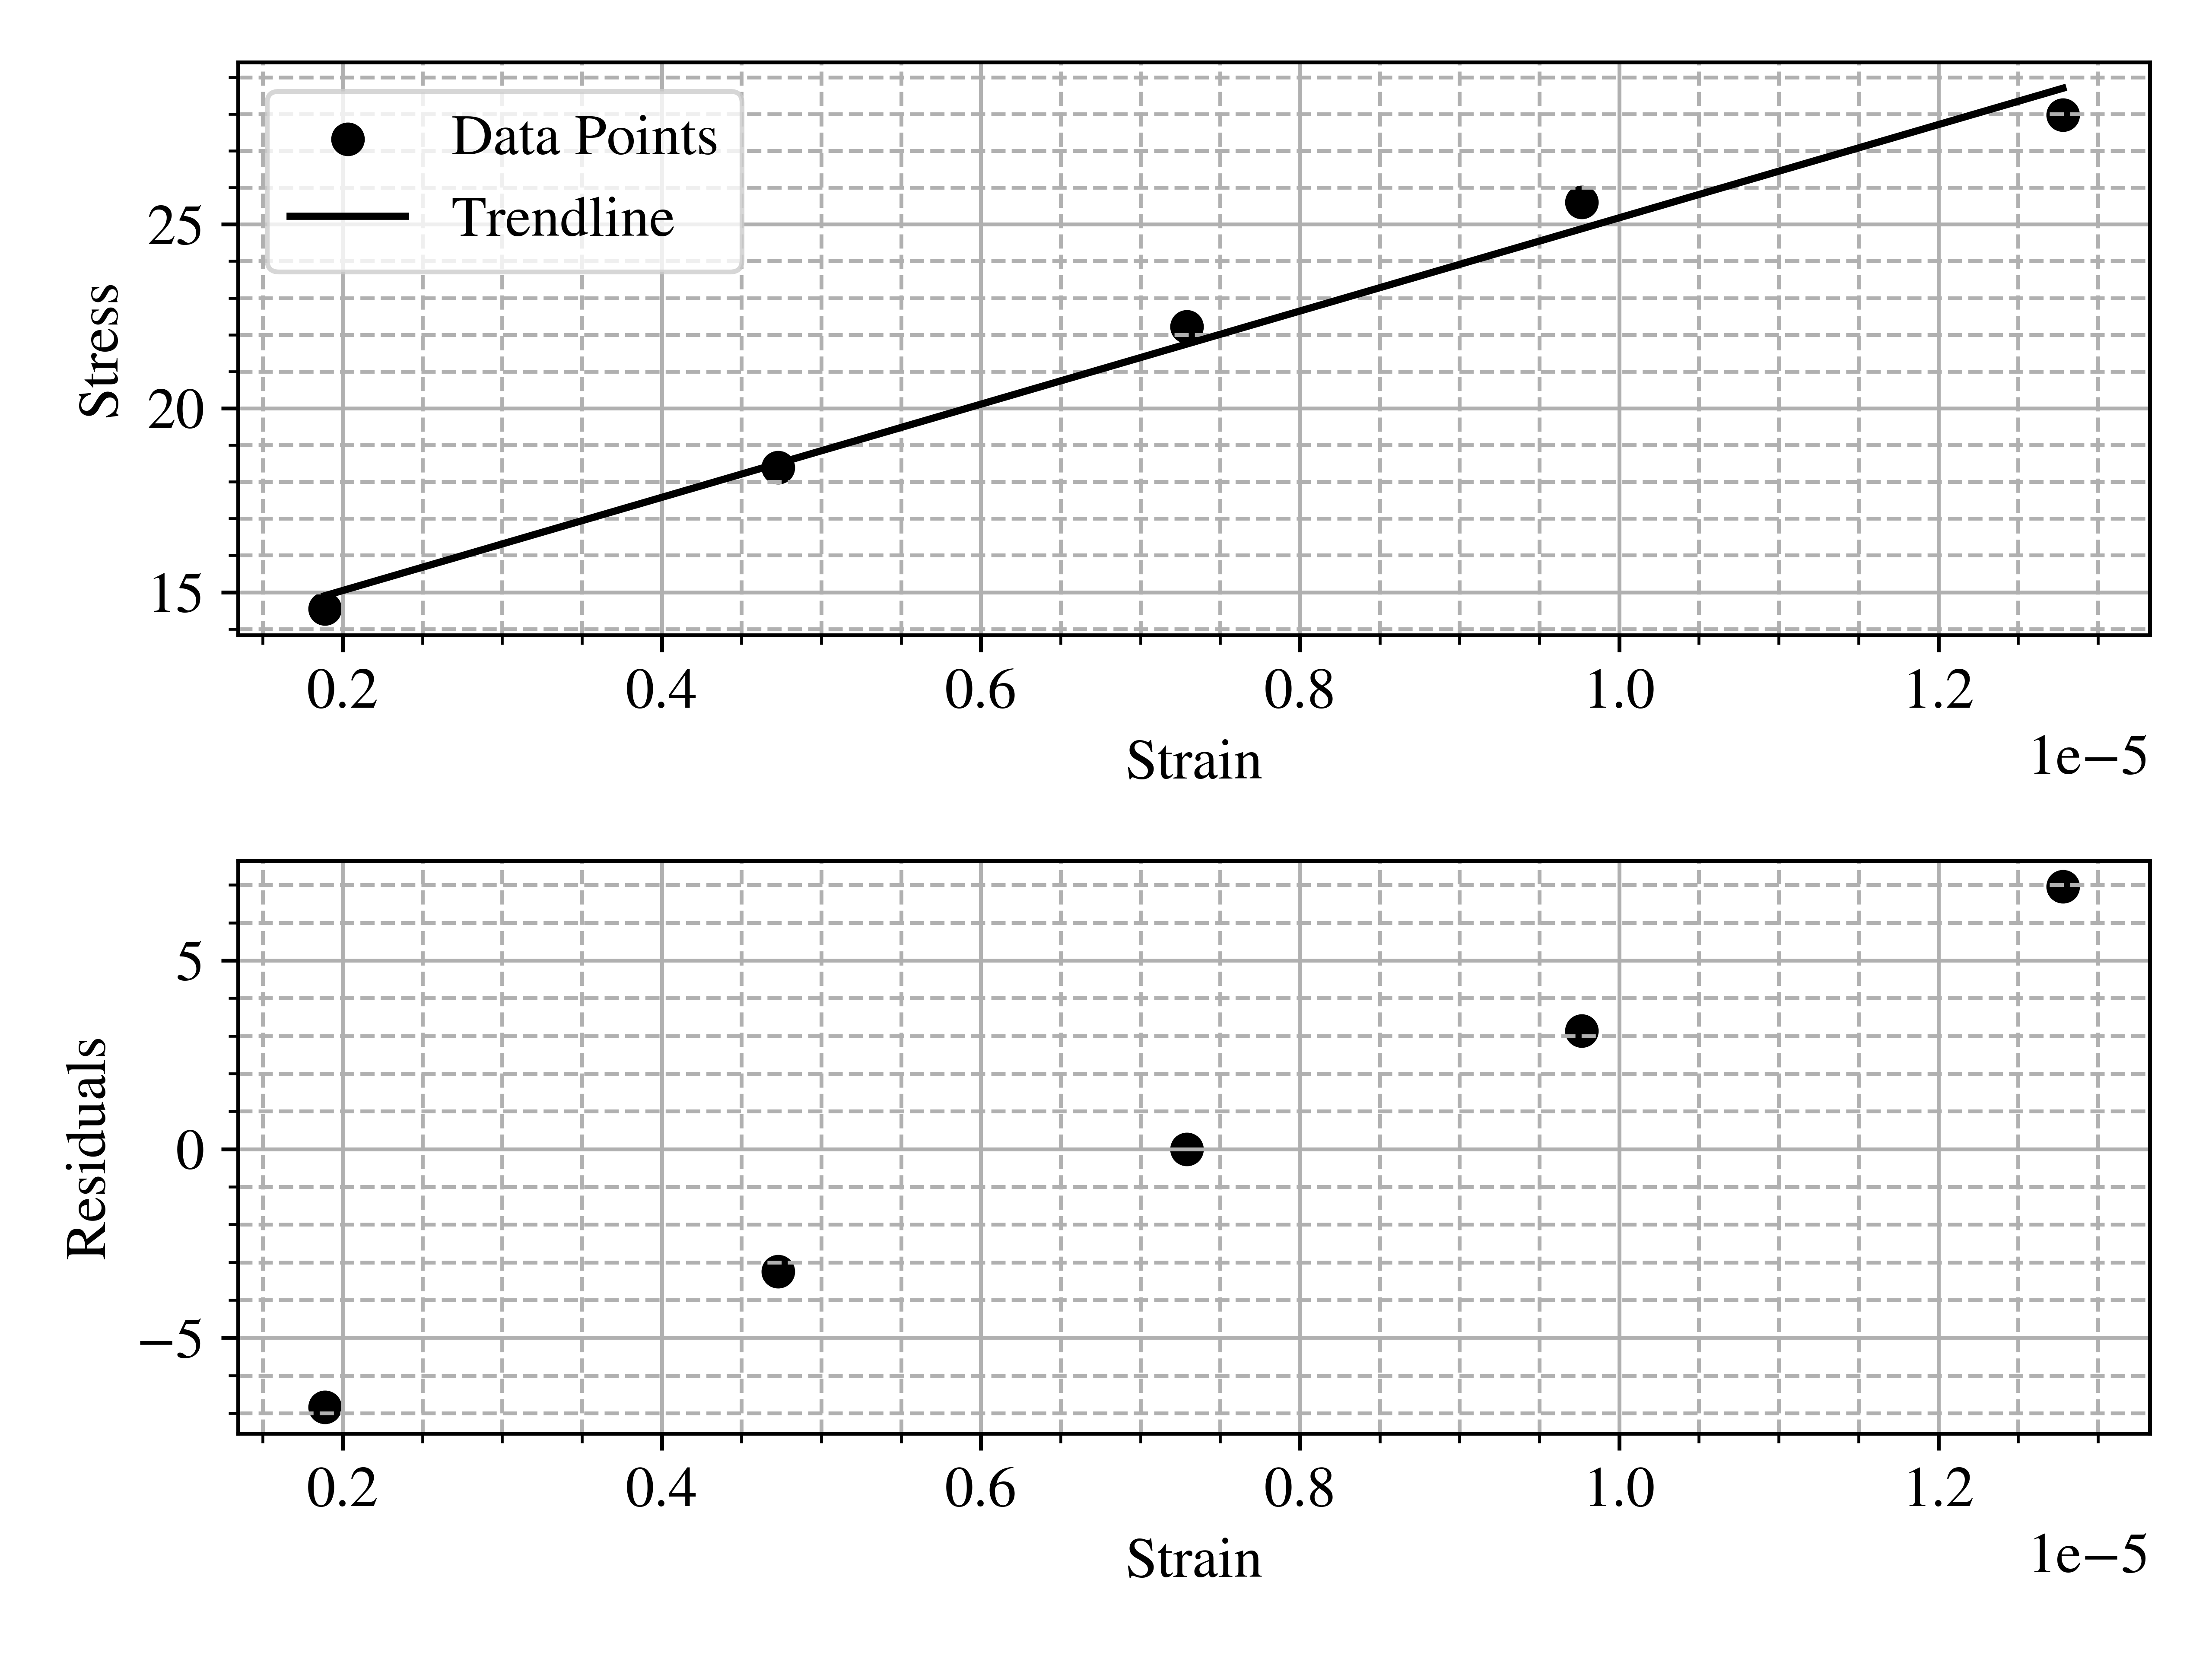
\includegraphics[width = 0.5\textwidth]{Plot1.png}\caption{A graph of the complex permittivity at each frequency for Methanol}\label{fig: Methanol Graph}
\end{figure}

\begin{figure}[H]
    \centering
    \includegraphics[width = 0.5\textwidth]{Plot2.png}\caption{A graph of the complex permittivity at each frequency for Sodium Chloride}\label{fig: NaCl Graph}
\end{figure}

\end{multicols*}

\section{References}
\printbibliography[heading = none]

\section{Appendix}
\begin{minted}{py}
import numpy as np
import pandas as pd
import matplotlib.pyplot as plt

# importing data to different dataframes for each sheet
data_air = pd.read_excel('Data.xlsx', 0)
data_short = pd.read_excel('Data.xlsx', 1)
data_water = pd.read_excel('Data.xlsx', 2)
data_methanol = pd.read_excel('Data.xlsx', 3).dropna()
data_NaCl = pd.read_excel('Data.xlsx', 4).dropna()
e_methanol = pd.read_excel('Data.xlsx', 5).dropna()
e_NaCl = pd.read_excel('Data.xlsx', 6).dropna()

# defining the frequency variable
frequency = np.array(data_air['%freq[Hz]'])

# finding the average of the real part of air
air_real_avg = data_air[['Real (S11) R1', 'Real (S11) R2', 'Real (S11) R3', 'Real (S11) R4' , 'Real (S11) R5', 'Real (S11) R6']].mean(axis=1)
data_air['Real Avg'] = air_real_avg

# finding the average of the imaginary part of air
air_imaginary_avg = data_air[['Imag (S11) R1', 'Imag (S11) R2', 'Imag (S11) R3', 'Imag (S11) R4' , 'Imag (S11) R5', 'Imag (S11) R6']].mean(axis=1)
data_air['Imag Avg'] = air_imaginary_avg

# finding the average of the real part of water
water_real_avg = data_water[['Real (S11) R1', 'Real (S11) R2', 'Real (S11) R3', 'Real (S11) R4' , 'Real (S11) R5', 'Real (S11) R6']].mean(axis=1)
data_water['Real Avg'] = water_real_avg

# finding the average of the imaginary part of water
water_imaginary_avg = data_water[['Imag (S11) R1', 'Imag (S11) R2', 'Imag (S11) R3', 'Imag (S11) R4' , 'Imag (S11) R5', 'Imag (S11) R6']].mean(axis=1)
data_water['Imag Avg'] = water_imaginary_avg

# finding the average of the real part of methanol
methanol_real_avg = data_methanol[['Real (S11) R1', 'Real (S11) R2', 'Real (S11) R3', 'Real (S11) R4' , 'Real (S11) R5', 'Real (S11) R6']].mean(axis=1)
data_methanol['Real Avg'] = methanol_real_avg

# finding the average of the imaginary part of methanol
methanol_imaginary_avg = data_methanol[['Imag (S11) R1', 'Imag (S11) R2', 'Imag (S11) R3', 'Imag (S11) R4' , 'Imag (S11) R5', 'Imag (S11) R6']].mean(axis=1)
data_methanol['Imag Avg'] = methanol_imaginary_avg

# finding the average of the real part of NaCl
NaCl_real_avg = data_NaCl[['Real (S11) R1', 'Real (S11) R2', 'Real (S11) R3', 'Real (S11) R4' , 'Real (S11) R5', 'Real (S11) R6']].mean(axis=1)
data_NaCl['Real Avg'] = NaCl_real_avg

# finding the average of the imaginary part of NaCl
NaCl_imaginary_avg = data_NaCl[['Imag (S11) R1', 'Imag (S11) R2', 'Imag (S11) R3', 'Imag (S11) R4' , 'Imag (S11) R5', 'Imag (S11) R6']].mean(axis=1)
data_NaCl['Imag Avg'] = NaCl_imaginary_avg

# finding the average of the given real permittivity of methanol
e_methanol_real_avg = e_methanol[["e'_R1","e'_R2","e'_R3"]].mean(axis=1)
e_methanol['Real Avg'] = e_methanol_real_avg

# finding the average of the given imaginary permittivity of methanol
e_methanol_imaginary_avg = e_methanol[["e''_R1","e''_R2","e''_R3"]].mean(axis=1)
e_methanol['Imag Avg'] = e_methanol_imaginary_avg

# finding the average of the given real permittivity of NaCl
e_NaCl_real_avg = e_NaCl[["e'_R1","e'_R2","e'_R3"]].mean(axis=1)
e_NaCl['Real Avg'] = e_NaCl_real_avg

# finding the average of the given imaginary permittivity of NaCl
e_NaCl_imaginary_avg = e_NaCl[["e''_R1","e''_R2","e''_R3"]].mean(axis=1)
e_NaCl['Imag Avg'] = e_NaCl_imaginary_avg

# defining the different perimittivity as numpy array
short_r_avg = data_short['re:Trc1_S11'].to_numpy()
short_i_avg = data_short['im:Trc1_S11'].to_numpy()

air_r_avg = data_air['Real Avg'].to_numpy()
air_i_avg = data_air['Imag Avg'].to_numpy()

water_r_avg = data_water['Real Avg'].to_numpy()
water_i_avg = data_water['Imag Avg'].to_numpy()

methanol_r_avg = data_methanol['Real Avg'].to_numpy()
methanol_i_avg = data_methanol['Imag Avg'].to_numpy()

NaCl_r_avg = data_NaCl['Real Avg'].to_numpy()
NaCl_i_avg = data_NaCl['Imag Avg'].to_numpy()

e_methanol_r_avg = e_methanol['Real Avg'].to_numpy()
e_methanol_i_avg = e_methanol['Imag Avg'].to_numpy()

e_NaCl_r_avg = e_NaCl['Real Avg'].to_numpy()
e_NaCl_i_avg = e_NaCl['Imag Avg'].to_numpy()

# creating the complex numbers from the averages
air_complex = air_r_avg - (1j * air_i_avg)
short_complex = short_r_avg - (1j * short_i_avg)
water_complex = water_r_avg - (1j * water_i_avg)
methanol_complex = methanol_r_avg - (1j * methanol_i_avg)
NaCl_complex = NaCl_r_avg - (1j * NaCl_i_avg)
e_methanol_c = e_methanol_r_avg - (1j * e_methanol_i_avg)
e_NaCl_c = e_NaCl_r_avg - (1j * e_NaCl_i_avg)

# calculating the different deltas required in the equation
delta_13 = np.subtract(short_complex, water_complex)
delta_21 = np.subtract(air_complex, short_complex)
delta_23 = np.subtract(air_complex, water_complex)
delta_32 = np.subtract(water_complex, air_complex)
delta_m1_methanol = np.subtract(methanol_complex, short_complex)
delta_m2_methanol = np.subtract(methanol_complex, air_complex)
delta_m3_methanol = np.subtract(methanol_complex, water_complex)
delta_m1_NaCl = np.subtract(NaCl_complex, short_complex)
delta_m2_NaCl = np.subtract(NaCl_complex, air_complex)
delta_m3_NaCl = np.subtract(NaCl_complex, water_complex)

# using the equation and values to calculate the complex permittivity
e_methanol = -1 * (((delta_m2_methanol * delta_13) / (delta_m1_methanol * delta_32)) * 80.5) - (((delta_m3_methanol * delta_21) / (delta_m1_methanol * delta_32)) * 1)
e_NaCl = -1 * (((delta_m2_NaCl * delta_13) / (delta_m1_NaCl * delta_32)) * 80.5) - (((delta_m3_NaCl * delta_21) / (delta_m1_NaCl * delta_32)) * 1)

# taking the real parts only
methanol_real = np.real(e_methanol)
e_methanol_real = np.real(e_methanol_c)
NaCl_real = np.real(e_NaCl)
e_NaCl_real = np.real(e_NaCl_c)

# polyfit calculated methanol
coefficients, cov = np.polyfit(frequency, methanol_real, 5, cov=True)
poly_function = np.poly1d(coefficients)
trendline_c_m = poly_function(frequency)

# polyfit given methanol
coefficients, cov = np.polyfit(frequency, e_methanol_real, 5, cov=True)
poly_function = np.poly1d(coefficients)
trendline_g_m = poly_function(frequency)

# polyfit calculated NaCl
coefficients, cov = np.polyfit(frequency, NaCl_real, 5, cov=True)
poly_function = np.poly1d(coefficients)
trendline_c_n = poly_function(frequency)

# polyfit given NaCl
coefficients, cov = np.polyfit(frequency, e_NaCl_real, 5, cov=True)
poly_function = np.poly1d(coefficients)
trendline_g_n = poly_function(frequency)

# value comparisons
positions = (0, 74, 174, 200)
for i in positions:
    print(f'The calculated permittivity at data point {i+1} for methanol is:{methanol_complex[i]:.2f}, while the given value is: {e_methanol_c[i]:.2f}')
    print(f'The calculated permittivity at data point {i+1} for NaCl is:{NaCl_complex[i]:.2f}, while the given value is: {e_NaCl_c[i]:.2f}')

# plotting the data for methanol
plt.figure(figsize=(7.5, 10.5))
plt.rcParams['font.family'] = 'STIXGeneral'
plt.rcParams['mathtext.fontset'] = 'stix'
plt.rcParams['font.size'] = 12
plt.rcParams['font.weight'] = 'normal'
plt.minorticks_on()
plt.grid(visible=True, which='major', linestyle='-')
plt.grid(visible=True, which='minor', linestyle='--')

plt.scatter(frequency, methanol_real, color='k', label='Calculated')
plt.plot(frequency, trendline_c_m, color = 'k', label='Calculated')
plt.scatter(frequency, e_methanol_real, color='grey', label='Given')
plt.plot(frequency, trendline_g_m, '--',  color = 'k', label = 'Given')
plt.xlabel('f/Hz')
plt.ylabel(r'$\mathrm{\epsilon_{methanol}}$')
plt.title('Complex Permittivity of Methanol vs Frequency')
plt.legend()
plt.savefig('Plot1.pdf', dpi=800)
plt.show()
plt.close()

# plotting the data of NaCl
plt.figure(figsize=(7.5, 10.5))
plt.rcParams['font.family'] = 'STIXGeneral'
plt.rcParams['mathtext.fontset'] = 'stix'
plt.rcParams['font.size'] = 12
plt.rcParams['font.weight'] = 'normal'
plt.minorticks_on()
plt.grid(visible=True, which='major', linestyle='-')
plt.grid(visible=True, which='minor', linestyle='--')

plt.scatter(frequency, NaCl_real, color='k', label='Calculated')
plt.plot(frequency, trendline_c_n, color = 'k', label='Calculated')
plt.scatter(frequency, e_NaCl_real, color='grey', label='Given')
plt.plot(frequency, trendline_g_n, '--',  color = 'k', label = 'Given')
plt.xlabel('f/Hz')
plt.ylabel(r'$\mathrm{\epsilon_{NaCl}}$')
plt.title('Complex Permittivity of NaCl vs Frequency')
plt.legend()
plt.savefig('Plot2.pdf', dpi=800)
plt.show()

\end{minted}


\end{document}